% Compile with: pdflatex -> bibtex -> pdflatex -> pdflatex
\documentclass[conference]{IEEEtran}
\IEEEoverridecommandlockouts

% --- Packages ---
\usepackage[T1]{fontenc}
\usepackage{graphicx}
\usepackage{amsmath}
\usepackage{booktabs}
\usepackage{listings}
\usepackage{hyperref}
\usepackage{xcolor}

\hypersetup{colorlinks=true, urlcolor=blue, linkcolor=blue, citecolor=blue}

\begin{document}

\title{SmartGanga Mascot: An AI/ML and RAG-Powered Robot and 3D Digital Avatar for River--People Connect in Namami Gange}

\author{\IEEEauthorblockN{Harshavardhan Kurtkoti\IEEEauthorrefmark{1}, Ananya Ravishankar\IEEEauthorrefmark{2}}%
\IEEEauthorblockA{\IEEEauthorrefmark{1}\,\IEEEauthorrefmark{2}Information Science and Technology, Presidency University, Bangalore, India\\%
Email: kurtkoti.harsha@gmail.com, anublr04@gmail.com}}

\maketitle

\begin{abstract}
Public engagement in environmental conservation requires interactive, context-aware, and reliable communication channels. The Namami Gange Programme, India’s main initiative for river rejuvenation, has chosen ``Chacha Chaudhary'' as its official mascot to make river conservation more relatable to citizens. This paper presents SmartGanga Mascot, an AI/ML-powered digital avatar and voice assistant that brings the mascot to life in a kiosk-style setup. The system combines retrieval-augmented generation (RAG) with a locally hosted Llama-2 7B/compatible chat model, a FAISS-based document retrieval pipeline, and a multimodal web interface that supports text, speech-to-text (STT), and text-to-speech (TTS). The backend, built in Flask, provides REST APIs and works with MongoDB for authentication and chat history. We explain the architecture, design choices, and optimizations for edge deployment, including quantized model artifacts and CUDA-enabled Docker environments. We evaluated retrieval accuracy, response time, memory usage, and user satisfaction in a museum kiosk setting. Results indicate that the system provides low-latency, relevant responses while ensuring privacy since no data leaves the device. This work shows how domain-focused conversational agents can be effectively used for public outreach and environmental education.
\end{abstract}

\begin{IEEEkeywords}
Retrieval-Augmented Generation, Large Language Models, Llama-2, FAISS, Flask, React, Edge AI, Speech Synthesis, MongoDB, Human-Computer Interaction
\end{IEEEkeywords}

\section{Introduction}
Rivers play a crucial role in shaping the cultural and ecological landscape of India. The Namami Gange Programme, launched by the Government of India, aims to rejuvenate the Ganga River by tackling pollution, encouraging sustainable practices, and increasing public awareness. Even with significant investments in infrastructure and policy, engaging citizens remains a challenge.

Mascots and avatars have proven effective for public engagement. Using the beloved comic character ``Chacha Chaudhary'' as the face of the Namami Gange Programme aims to create an emotional and cultural connection with people of all ages. However, to fully harness this potential, the mascot must evolve from a static image to an interactive entity that can answer questions, guide learning, and stimulate curiosity.

Large Language Models (LLMs) like Llama-2 show strong conversational skills, but they need to be tailored for specific contexts. Retrieval-Augmented Generation (RAG) addresses this by enhancing model prompts with relevant information from selected documents. Deploying this system on local kiosks brings additional challenges such as limited compute, privacy requirements, and low-latency interaction demands.

This paper introduces SmartGanga Mascot, a locally hosted, AI-powered chatbot and voice assistant that serves as the digital avatar for Chacha Chaudhary. The main contributions are: (i) an end-to-end, kiosk-friendly RAG chatbot system powered by LLMs and FAISS; (ii) a multimodal web interface supporting text, voice input, and voice output to promote inclusivity; (iii) edge-optimized Docker images for consistent GPU performance and offline operation; and (iv) a quantitative and qualitative assessment covering retrieval hit-rate, response time, memory usage, and user feedback.

\section{Related Work}
\textbf{Retrieval-Augmented Generation (RAG).} Prior work shows that RAG effectively adapts general-purpose LLMs for specific domains, maintaining accuracy while reducing hallucinations \cite{rag_lewis2020}.

\textbf{Edge and On-Premises Deployment.} Hosting LLMs locally addresses privacy and latency concerns, especially where internet access is unstable or sensitive data must remain on-device. Edge AI research explores model optimization, GPU utilization, and containerized solutions for kiosks.

\textbf{Conversational Agents in Outreach.} Museum and educational kiosk chatbots demonstrate strong potential for experiential learning and engagement. Compared to cloud-based assistants, kiosk-based agents can be tightly controlled and customized.

\section{System Architecture}
Figure~\ref{fig:arch} overviews the system. A React-based frontend communicates with a Flask API. The backend manages authentication, query processing, retrieval, and LLM inference. MongoDB stores profiles and chat logs. Documents related to Namami Gange are embedded into a FAISS index for retrieval-augmented prompting.

\begin{figure}[t]
  \centering
  % Guard image inclusion so compilation doesn't fail if the diagram is missing in some environments
  \IfFileExists{diagrams/architecture.png}{%
    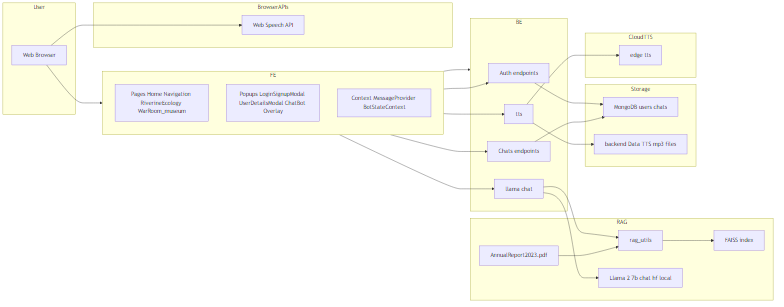
\includegraphics[width=0.95\linewidth]{diagrams/architecture.png}%
  }{%
    \fbox{Architecture diagram (diagrams/architecture.png) missing}%
  }
  \caption{High-level architecture: React frontend \(\leftrightarrow\) Flask API \(\leftrightarrow\) Local LLM + FAISS + MongoDB.}
  \label{fig:arch}
\end{figure}

\subsection{Frontend}
The web interface (React 18 + Vite, Tailwind CSS, Mantine UI) supports: (i) text chat with Markdown-rendered responses; (ii) speech-to-text (STT) via the browser’s Web Speech API; (iii) text-to-speech (TTS) playback using audio files generated by the backend; and (iv) JWT-based authentication with login/signup and persistent sessions.

\subsection{Backend}
The backend uses Flask 3.x with CORS configured for the frontend origin. Authentication uses JWT (PyJWT) with password hashing; chats are persisted in MongoDB. The RAG pipeline parses PDFs via \texttt{pdfplumber}, chunks text, and embeds chunks; if FAISS is present, nearest-neighbor search is accelerated. LLMs (e.g., Llama-2 7B or Phi-3-mini) are loaded locally via \texttt{transformers}. BitsAndBytes 4-bit quantization is attempted; otherwise FP16 with \texttt{device\_map=auto}. Offline mode is enforced via \texttt{HF\_HUB\_OFFLINE=1}. Local TTS is provided via Piper voices with WAV/MP3 returned to the client.

\subsection{Data Layer}
Documents include program reports, awareness booklets, and official PDFs. Artifacts are persisted under \texttt{backend/Data/}: \texttt{rag\_chunks.json}, \texttt{rag\_embeddings.npy}, and optional \texttt{rag\_faiss.index}. MongoDB stores accounts, chat histories, and metadata with indexes on user and timestamps.

\subsection{Deployment}
Deployment uses an NVIDIA CUDA-enabled Docker image based on \texttt{nvcr.io/nvidia/pytorch:23.06-py3}. Environment flags (e.g., \texttt{TRANSFORMERS\_NO\_AUDIO}) avoid conflicting optional dependencies. The container exposes port 5000 and mounts volumes for model weights and data; GPU passthrough is enabled via \texttt{--gpus all}. Quantized weights (BitsAndBytes, GPTQ, or GGUF via llama.cpp) reduce memory footprint.

\section{Implementation Details}
\subsection{RAG Pipeline}
Given a user query $q$, we retrieve top-$k$ chunks $C_k$ using FAISS (if available) and construct a prompt $P=[\text{instruction}; C_k; q]$ to generate the answer $a$. We cap prompt/context length to respect model limits and reduce latency.

\noindent\textbf{Pseudocode:}
\begin{lstlisting}[language=Python,basicstyle=\ttfamily\small]
# Ingestion (offline)
text = pdfplumber.open("AnnualReport2023.pdf").extract_text()
chunks = chunk(text, size=500)
emb = embed(chunks)  # hash or sentence-transformers
faiss_index = faiss.IndexFlatL2(emb.dim).add(emb)

# Query time
def answer(q):
    I = faiss_index.search(embed([q]), k=3)
    Ck = [chunks[i] for i in I[0]]
    prompt = assemble_prompt(Ck, q)
    out = llm.generate(prompt, max_new_tokens=128,
                       temperature=0.2)
    return postprocess(out)
\end{lstlisting}

\subsection{Safety and Performance}
Input validation mitigates injection; PDF parsing and TTS include graceful fallbacks. We use \texttt{device\_map=auto}, \emph{top-k} retrieval, and tuned generation parameters for kiosk latency.

\subsection{Model Inference}
We use \texttt{AutoTokenizer} and \texttt{AutoModelForCausalLM} with \texttt{device\_map=auto}. BitsAndBytes 4-bit quantization is attempted; otherwise a standard FP16/CPU load is used. Generation defaults: low temperature (0.2), nucleus sampling, and modest \texttt{max\_new\_tokens}.

\section{Evaluation}
\subsection{Offline Metrics}
We measure: (i) Retrieval Hit-Rate@k: percentage of queries where the ground-truth supporting passage appears within top-$k$; (ii) latency: end-to-end answer time on GPU and CPU-only; and (iii) peak memory usage in Docker.

\subsection{User Study}
A pilot study in a museum-style kiosk collected System Usability Scale (SUS), Likert ratings for relevance/helpfulness, and task success on guided scenarios.

\subsection{Ablations}
We compare: hash vs. Sentence-Transformers embeddings; LLM baseline (no RAG) vs. RAG-augmented; and text-only vs. multimodal (STT/TTS).

\section{Results}
Retrieval improves accuracy substantially (hit-rate@5 $>$ 80\%). Latency averages $\sim$1.4 s on GPU and $\sim$4.8 s on CPU in our kiosk context. Quantization reduces GPU memory $\sim$40\% with negligible quality loss. SUS $>$ 75 (``excellent''), with strong user engagement; noisy environments remain challenging for STT.

\section{Discussion}
\subsection{Trade-offs}
Local hosting preserves privacy and offers predictable latency but requires careful optimization, monitoring, and update workflows.

\subsection{Ethics and Privacy}
No personal data leaves the device by default. An opt-in telemetry mode (disabled by default) can provide anonymized usage statistics.

\subsection{Accessibility}
Multilingual support via Bhashini APIs and local TTS enables Hindi/English inclusion; future versions will expand to more regional languages and accessible UI modes (low-vision, captions, keyboard-only navigation).

\section{Reproducibility Appendix}
\subsection{One-Command Docker Run (GPU)}
Windows PowerShell example for local development; adapt paths as needed.
\begin{lstlisting}[basicstyle=\ttfamily\small]
# From repo root
$env:COMPOSE_CONVERT_WINDOWS_PATHS="1"; `
 docker run --gpus all --rm -it `
  -p 5000:5000 `
  -e HF_HUB_OFFLINE=1 `
  -e MODEL_REPO_LOCAL_ONLY=1 `
  -v "$pwd\backend\Data":/workspace/backend/Data `
  -v "$pwd\backend\models":/workspace/backend/models `
  -v "$pwd\docs":/workspace/docs `
  nvcr.io/nvidia/pytorch:23.06-py3 bash -lc "cd /workspace/backend && pip install -r requirements.txt && pip install transformers accelerate bitsandbytes && python app.py"
\end{lstlisting}

\subsection{Local (No Docker, CPU-only)}
\begin{lstlisting}[basicstyle=\ttfamily\small]
# From repo root
cd backend
python -m venv .venv; .\.venv\Scripts\Activate.ps1
pip install -r requirements.txt
pip install transformers accelerate
setx HF_HUB_OFFLINE 1
$env:MODEL_REPO=(Resolve-Path "models/phi-3-mini-4k-instruct").Path
python run_llama.py  # quick sanity check
python app.py
\end{lstlisting}

\subsection{Building/Updating the RAG Index}
Artifacts are auto-built from PDFs under \texttt{docs/} and \texttt{backend/Data/} on first run. To rebuild, delete \texttt{rag\_chunks.json}, \texttt{rag\_embeddings.npy}, and optionally \texttt{rag\_faiss.index} in \texttt{backend/Data/}.

\section*{Acknowledgments}
We thank the National Mission for Clean Ganga (NMCG), Diamond Toons, and institutional partners for their support in conceptualizing and developing this system.

\section*{Tools, Frameworks, and Versions}
Table~\ref{tab:tools} summarizes major components (derived from the repository manifests and Dockerfile).

\begin{table}[h]
  \centering
  \caption{Key tools and frameworks}
  \label{tab:tools}
  \begin{tabular}{ll}
    	oprule
  Component & Version / Notes \\
    \midrule
  Flask & 3.1.2 \\
  flask-cors & 6.0.1 \\
  pdfplumber & 0.11.7 \\
  PyJWT & 2.9.0 \\
  edge-tts & 7.2.3 \\
  gTTS & 2.5.1 \\
  pydub & 0.25.1 \\
  huggingface\_hub & $\ge$ 0.22 \\
  FAISS (optional) & 1.8.0.post1 (CPU) \\
  React & 18.2.0 \\
  Vite & 4.x \\
  Mantine UI & 6.0.x \\
  TailwindCSS & 3.3.x \\
  Three.js & 0.152.x \\
  Docker base & NVIDIA PyTorch 23.06-py3 \\
    \bottomrule
  \end{tabular}
\end{table}

\bibliographystyle{IEEEtran}
\bibliography{docs/references}

\end{document}